\section{Our Approach}
%\label{sec:approach}
Given multiple overlapping images of an indoor scene from different views, our approach produces the combined room layout represented by several room corners, as shown in Fig. \ref{fig:partial1}. When the overall FOV of the multi-view images contains the entire room, we can recover the whole-room layout, better viewed in panorama, Fig. \ref{fig:results2}. 
%
The algorithm pipeline is shown in Fig. \ref{fig:overview}. First, we estimate the partial room layout separately in each image using an encoder-decoder structure, as described in Sec. \ref{sec:layout}. Then the estimated partial room layouts are integrated into a combined probability map, based on the view transformations. 
We \xj{simply average?} use a linear blending to average the predictions from different views, and select the points of the maximum responses as the room corners, as described in Sec. \ref{sec:merging}. 

\comments{
We further align the panorama to be level with \xj{(what do you mean by be level with?)} the floor and reconstruct 3D structure of the room, as described in Sec.~\ref{sec:align}. 
}

\begin{figure*}[ht]
	\centering
	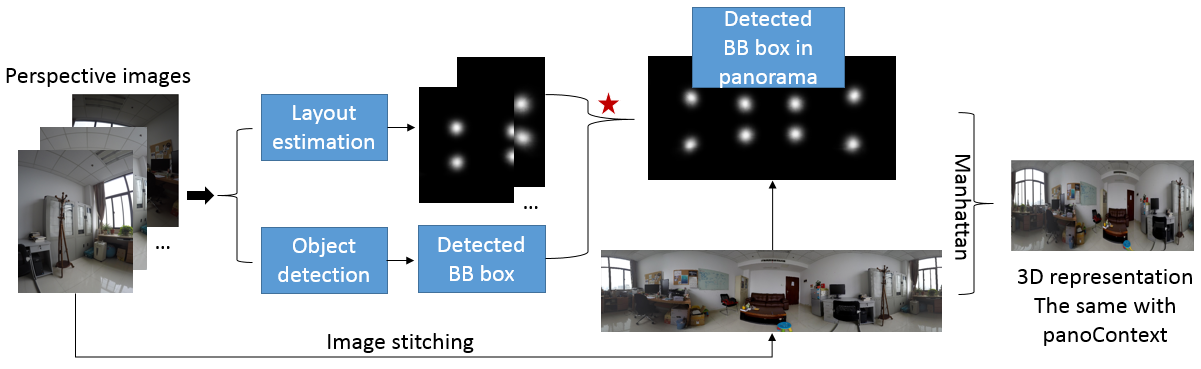
\includegraphics[width=\linewidth]{figs/ppline.png}
	\caption{System overview. }
	\label{fig:overview}
\end{figure*}

\subsection{Single-view room Layout Estimation}
\label{sec:layout}

Many methods have been proposed to estimate the room layout from a single RGB image. 
%In this section, we are going to recover the room layout for perspective images from different views. 
Previous DNN-based techniques of room layout estimation typically represent the room layout as a segmentation of semantic surfaces including walls, ceilings and floors~\cite{dasgupta2016delay, ours} or as the semantic boundaries or intersection points among them \cite{ren2016coarse}. 
%
These representations have proved valid and reasonable. However, due to the overlaps across views, they all carry too much redundant predictions and are inconvenient for combination under the circumstances of multi-view layout estimation. Out of this reason, we propose the \emph{secondary representation} of a room layout.
%
%A direct way to achieve our goal is to utilize existing methods to estimate the layout for each view, and then combine these representations to produce the complete-room 3D layout. 
%However, this method is not efficient due to many redundant predictions caused by overlaps across views. 
\comments{
To avoid redundant predictions or even to benefit from them, we propose a \emph{secondary representation} of a room layout on perspective images. The room layout under each view is only represented by the intersections of vertical walls and ceiling or floor. We call these intersections secondary keypoints. 
\xj{What about the case when there in only one wall surface?}
Obviously, without the extra intersections of two semantic planes on the image boundaries, we cannot recover the room layout from a single perspective. However, these secondary keypoints in overlapping views are sufficient to reconstruct the 3D layout of the entire room. Compared to previous representations, our secondary keypoints are quite simplified and easier to train. It also naturally avoids a lot of redundant predictions. 
}

\paragraph{Layout Representation.}
\xj{Explain more details of this new representation: add a figure. and more constraints? say, there are at most four points on each image? Split them to upper/lower parts?}
Under the Manhattan world assumption \cite{coughlan1999manhattan}, a 3D room can be modeled as a cube. The room layout in a single view is then the projection of this cube. As the cube can be defined by its 8 vertices, we adopt the location of these vertices, so called room corners, on the projected images to represent the room layout. Intuitively, there should be 0 to 4 room corners in a single-view image. 
%
Motivated by \cite{LeeRoomNet17} and the studies on human pose estimation \cite{tompson2014joint,pfister2015flowing}, we further formulate the room corners on the image plane as 2D Gaussian centered at their locations. The standard deviation is set to 40 pixels in our case.
%
Considering the inherent semantic differences, we classify the room corners into two categories: the upper room corner which is the intersection of two walls and ceiling, and the lower room corner which is the intersection of two walls and floor. In consequence, the goal of the single-view net should be estimating the probability maps of these two kinds of room corners for the input image, as depicted in Fig. \ref{fig:network}.
%
Compared to previous representations, our \emph{secondary representation} is quite simplified and easier to train. It also naturally avoids a lot of redundant predictions. 

 
%We use an encoder-decoder Network structure proposed in \cite{RoomNet} to estimate room layouts on perspective images. The room layout is represented by a series of keypoints in a particular order. The keypoints are the intersection of different semantic planes on the the perspective images. By learning the location of these keypoints, a room layout can be reconstructed by simply connect these keypoints in a specific order.

\noindent\textbf{Network Architecture.} We adopt the encoder-decoder architecture proposed by \cite{LeeRoomNet17} with modifications, \xj{since it is an end-to-end framework without any post-processing} since it can serve as an end-to-end framework that do not need complex post-processing. 
%
The modified network architecture, called SVNet, is shown in Fig.~\ref{fig:network}. It is designed to estimate the room corners in a single-view image. 
%Our network for room corner estimation from a single-view image is shown in Fig.~\ref{fig:network}.
\xj{We mainly make two modifications: decode part and classfication branch.} 
We mainly make two modifications: decode part and classfication branch. Firstly, as our secondary representation is easier to learn, we remove the recurrent structure in \cite{LeeRoomNet17} for efficiency, and then we add more upsampling layers and convolution layers to upsample the feature maps from the bottleneck layer to full input resolution as compensation for accuracy. The final convolution layer is adapted to output a $w \times h \times 2$ probability array $T$ for our new representation, where $w$ and $h$ stand for the width and length of the input image. Each of the 2 slices can be viewed as a probability map for the room corners in the corresponding category. Secondly, 
\cite{LeeRoomNet17} delineate room layout using 2D keypoints. The semantic boundaries can be recovered by connecting the detected 2D keypoints in a specific order. As the connection order differs between room topologies, they have to add a classification branch in their network to classify the room type, and the final performance rely on the classification accuracy. Unfortunately, the accuracy is not so well. We naturally avoid this awkward situation by using our \emph{secondary representation}. The simplified representation divides the room corners into only two categories and applies to all room types. So we elegantly remove the classification branch in our network architecture.

%First, the encoder part consists of 13 convolutional layers, which are topologically identical to the VGG16 network. It encodes the $320\times320$ input images to $10\times10$ feature maps. 
\comments{
We modify the decoder part to upsample the feature maps from the bottleneck layer with low resolution to full input resolution. \xj{what is the original decoder?}
%
Second, we remove the classification branch of the original RoomNet because our simplified representation is consist for different topology of visible surfaces in the scene. 
\xj{Therefore, our network outputs ... ?}
}

\begin{figure}
	\centering
	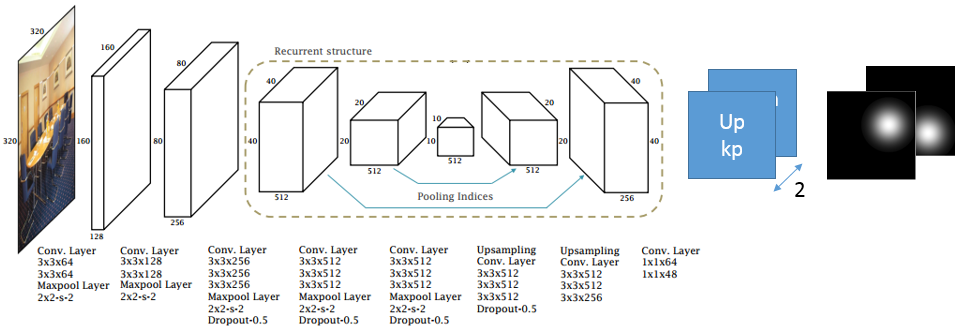
\includegraphics[width=\linewidth]{figs/network.png}
	\caption{Network architecture. }
	\label{fig:network}
\end{figure}

\noindent\textbf{Training.} 
We adopt the PanoContext dataset \cite{zhang2014panocontext} (and relabeled Stanford 2D-3D dataset \cite{layoutnet}) to generate multi-view images for training. The PanoContext dataset contains 500 annotated panoramic images. We project these panorama into multiple $320 \times 320$ images at different views using the toolkit provided by \cite{zhang2014panocontext}. The ground truth locations of the room corners are obtained using the same transformations and are further transformed into the Gausian representation. At training stage, Euclidean loss is used as the cost function to regress the probability map of room corners. As the area of the background is much larger than the foreground in the Gausian ground truth, we adjust the distribution imbalance between foreground and background pixels by degrading the gradient weight of background pixels with a coefficient of 0.2.

%To obtain multiple overlapping perspective images, we project the panoramic images into different views using the toolkit provided by \cite{pano}. The ground truth of the secondary keypoints is represented by several 2D Gaussian heatmaps centered at their locations. We adjust the distribution imbalance between foreground and background pixels by degrading the gradient weight of background pixels with a coefficient of 0.2.

%The RoomNet-basic struture in \cite{RoomNet} is adopted in our training stage for efficiency. We first pretrain the Network on LSUN \cite{LSUN2016} training set. Then, to finetune the model on images from different views in the same room, we project the panorama from \cite{PanoContext} to $k$ views. We set $k$ to 12 and 24 in our experiment. The layout ground truth is relabeled using the same projection. 

%The secondary keypoints can be divided into two categories according to semantics: the intersection of two walls and ceiling or the intersection of two walls and floor.\xj{Move this sentence to the representation paragraph.}

%We train the network to regress these two kinds of keypoints separately in order to eliminate the ambiguity between them. For this reason, the output of our network is a $w \times h \times 2$ probability array $T$, where $w$ and $h$ stand for the width and length of the input image. Each of the 2 slices can be viewed as a probability map for the secondary keypoints in a corresponding category. 


\subsection{Layout composition}
\label{sec:merging}
In this section, we composite the predicted layouts from different perspectives and generate a combined layout estimation. First, the input multi-view images are projected into a combined image using the camera poses, we formulate this view transformations as a function $f$. Then, we sum over the third dimension of the probability array $T$ for each image to get a heatmap $\hat{T}$ depicting all included room corners. Next, we use the same mapping $f$ to map the heatmap $\hat{T}$ from different views into a combined predictions. A linear blending along horizontal lines is applied to average the predictions of the overlapping area between different views, as shown in Fig. \ref{fig:blending}. 

%
After that, what we are going to do is picking the points of the maximum responses as the room corners. At this stage, we first reduce the noise in $\hat{T}$ caused by unsatisfactory predictions from particular perspectives. We calculate the LOG response of $\hat{T}$ at a certain scale (depending on the radius of the room corners), $\sigma$ is set to 21 in our case, and use the LOG response as our new heatmap.
%
Then, we follow the post-processing method in \cite{zou2018layoutnet} to obtain the locations of the room corners in the combined heatmap. In brief, the combined heatmap is summed across rows to find $m$ local maxima for columns, then $n$ largest peaks are found along each of the $m$ columns. In this way, we attain the locations of $m \times n$ room corners. In the case of panorama, $m$ is set to 4 and $n$ is set to 2. The whole room layout can be reconstructed by connecting these eight keypoints. 

\begin{figure}
	\centering
	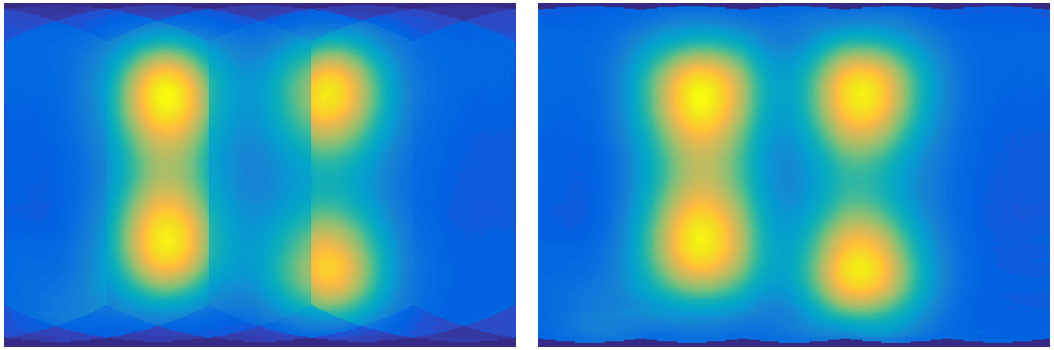
\includegraphics[width=\linewidth]{figs/blending.png}
	\caption{The combined probability map. Using simply average (left) or linear blending along horizontal lines (right).}
	\label{fig:blending}
\end{figure}


\comments{
\subsection{Alignment and 3D Reconstruction}
\label{sec:align}

(Optional and undone) In this section, we align the panoramic images to make sure that wall-wall boundaries are vertical to the floor. If we use the panorama to generate testing images, this step can be omitted as the reprojected panoramic images naturally met this alignment condition. Then the aligned panorama can be further rendered into a 3D representation. These two steps are implemented using existing techniques but the rendering part is not yet available. 
}
